\chapterimage{chapter-bg.png} % Chapter heading image

\chapter{Advanced Use}\label{advanced-use}

\section{Files and Directories}\label{files-and-directories}

Stellarium has many data files containing such things as star catalogue
data, nebula images, button icons, font files and configuration files.
When Stellarium looks for a file, it looks in two places. First, it
looks in the \emph{user directory} for the account which is running
Stellarium. If the file is not found there, Stellarium looks in the
\emph{installation directory}\footnote{The installation directory was
  referred to as the config root directory in previous versions of this
  guide}. Thus it is possible for Stellarium to be installed as an
administrative user and yet have a writable configuration file for
non-administrative users. Another benefit of this method is on
multi-user systems: Stellarium can be installed by the administrator,
and different users can maintain their own configuration and other files
in their personal user accounts.

In addition to the main search path, Stellarium saves some files in
other locations, for example screens shots and recorded scripts.

The locations of the user directory, installation directory,
\emph{screenshot save directory} and \emph{script save directory} vary
according to the operating system and installation options used. The
following sections describe the locations for various operating systems.

\subsection{Windows}\label{windows}

\begin{itemize}
\item
  \textbf{installation directory} By default this is
  \texttt{C:\textbackslash{}Program\ Files\textbackslash{}Stellarium\textbackslash{}},
  although this can be adjusted during the installation process.
\item
  \textbf{user directory} This is the Stellarium sub-folder in the
  Application Data folder for the user account which is used to run
  Stellarium. Depending on the version of Windows and its configuration,
  this could be any of the following (each of these is tried, if it
  fails, the next in the list if tried).
\end{itemize}

\texttt{\%APPDATA\%\textbackslash{}Stellarium\textbackslash{}}\\
\texttt{\%USERPROFILE\%\textbackslash{}Stellarium\textbackslash{}}\\
\texttt{\%HOMEDRIVE\%\textbackslash{}\%HOMEPATH\%\textbackslash{}Stellarium\textbackslash{}}\\
\texttt{\%HOME\%\textbackslash{}Stellarium\textbackslash{}}\\
\texttt{Stellarium\textbackslash{}s~installation~directory}


Thus, on a typical Windows XP system with user ``Bob Dobbs'', the user
directory will be:

\texttt{C:\textbackslash{}Documents~and~Settings\textbackslash{}Bob~Dobbs\textbackslash{}Application~Data\textbackslash{}Stellarium\textbackslash{}}

Thus, on a typical Windows Vista and Windows 7 systems with user ``Bob
Dobbs'', the user directory will be:

\texttt{C:\textbackslash{}Users\textbackslash{}Bob~Dobbs\textbackslash{}AppData\textbackslash{}Roaming\textbackslash{}Stellarium\textbackslash{}}

Stellarium version 0.9.0 did use the
\texttt{\%APPDATA\%\textbackslash{}Stellarium} folder. Thus if a
\texttt{config.ini} file exists in the
\texttt{\%USERPROFILE\%\textbackslash{}Stellarium\textbackslash{}}
directory, that will be used in preference to the
\texttt{\%APPDATA\%\textbackslash{}Stellarium\textbackslash{}}
directory. This is to prevent users of version 0.9.0 from losing their
settings when they upgrade.

\begin{itemize}
\item
  \textbf{screenshot save directory} Screenshots will be saved to the
  Desktop, although this can be changed with a command line option (see
  section \href{Advanced_Use\#Command_Line_Options}{Command Line
  Options}\footnote{Windows Vista users who do not run Stellarium with
    administrator priviliges should adjust the shortcut in the start
    menu to specify a different directory for screenshots as the Desktop
    directory is not writable for normal progams. The next release of
    Stellarium will include a GUI option to specify the screenshot
    directory.}).
\end{itemize}

\subsection{Mac OS X}\label{mac-os-x}

\begin{itemize}
\item
  \textbf{installation directory} This is found inside the application
  bundle, \texttt{Stellarium.app}. See the
  \href{http://www.mactipsandtricks.com/articles/Wiley_HT_appBundles.lasso}{Inside
  Application Bundles} for more information.
\item
  \textbf{user directory} This is the
  \texttt{Library/Preferences/Stellarium/} (or
  \texttt{\textasciitilde{}/Library/Application\ Support/Stellarium} on
  newest versions of Mac OS X) sub-directory of the users home
  directory.
\item
  \textbf{screenshot save directory} Screenshots are saved to the users
  Desktop.
\end{itemize}

\subsection{Linux}\label{linux}

\begin{itemize}
\item
  \textbf{installation directory} This is in the
  \texttt{share/stellarium} sub-directory of the installation prefix,
  i.e. usually \texttt{/usr/share/stellarium} or
  \texttt{/usr/local/share/stellarium/}.
\item
  \textbf{user directory} This is the \texttt{.stellarium} sub-directory
  of users home directory, i.e. \texttt{\textasciitilde{}/.stellarium/}.
\item
  \textbf{screenshot save directory} Screenshots are saved to the users
  home directory.
\end{itemize}

\subsection{Directory Structure}\label{directory-structure}

Within the \emph{installation directory} and \emph{user directory}
(defined in section \href{Advanced_Use\#Files_and_Directories}{Files and
Directories}), files are arranged in the following sub-directories.

\begin{itemize}
\item
  \textbf{landscapes/} contains data files and textures used for
  Stellarium's various landscapes. Each landscape has it's own
  sub-directory. The name of this sub-directory is called the
  \emph{landscape ID}, which is used to specify the default landscape in
  the main configuration file.
\item
  \textbf{skycultures/} contains constellations, common star names and
  constellation artwork for Stellarium's many sky cultures. Each culture
  has it's own sub-directory in the skycultures directory.
\item
  \textbf{nebulae/} contains data and image files for nebula textures.
  In future Stellarium will be able to support multiple sets of nebula
  images and switch between them at runtime. This feature is not
  implemented for version 0.9.1, although the directory structure is in
  place - each set of nebula textures has it's own sub-directory in the
  nebulae directory.
\item
  \textbf{stars/} contains Stellarium's star catalogues. In future
  Stellarium will be able to support multiple star catalogues and switch
  between them at runtime. This feature is not implemented for version
  0.10.0, although the directory structure is in place - each star
  catalogue has it's own sub-directory in the stars directory.
\item
  \textbf{data/} contains miscellaneous data files including fonts,
  solar system data, city locations etc.
\item
  \textbf{textures/} contains miscellaneous texture files, such as the
  graphics for the toolbar buttons, planet texture maps etc.
\end{itemize}

If any file exists in both the installation directory and user
directory, the version in the user directory will be used. Thus it is
possible to override settings which are part of the main Stellarium
installation by copying the relevant file to the user area and modifying
it there.

It is also possible to add new landscapes by creating the relevant files
and directories within the user directory, leaving the installation
directory unchanged. In this manner different users on a multi-user
system can customise Stellarium without affecting the other users.

\section{The Main Configuration
File}\label{the-main-configuration-file}

The main configuration file is read each time Stellarium starts up, and
settings such as the observer's location and display preferences are
taken from it. Ideally this mechanism should be totally transparent to
the user - anything that is configurable should be configured ``in'' the
program GUI. However, at time of writing Stellarium isn't quite complete
in this respect, despite improvements in version 0.10.0. Some settings
can only be changed by directly editing the configuration file. This
section describes some of the settings a user may wish to modify in this
way, and how to do it.

If the configuration file does not exist in the \emph{user directory}
when Stellarium is started (e.g. the first time the user starts the
program), one will be created with default values for all settings
(refer to section \href{Advanced_Use\#Files_and_Directories}{Files and
Directories} for the location of the user directory on your operating
system). The name of the configuration file is
\texttt{config.ini}\footnote{It is possible to specify a different name
  for the main configuration file using the \texttt{-\/-config-file}
  command line option. See section
  \href{Advanced_Use\#Command_Line_Options}{Command Line Options} for
  details.}.

The configuration file is a regular text file, so all you need to edit
it is a text editor like \emph{Notepad} on Windows, \emph{Text Edit} on
the Mac, or \emph{nano/vi/gedit} etc. on Linux.

The following sub-sections contain details on how to make commonly used
modifications to the configuration file. A complete list of
configuration file options and values may be found in the appendix,
\href{Configuration_file}{Configuration file}.

\section{Command Line Options}\label{command-line-options}

Stellarium's behaviour can be modified by providing parameters to the
program when it is run, via the command line. See table for a full list:

\begin{longtabu} to \textwidth {l|l|X}
\toprule
\emph{Option} & \emph{Option Parameter} & \emph{Description}\tabularnewline
\midrule
-\/-help or -h & {[}none{]} & Print a quick command line help message
and exit. \tabularnewline
\midrule
-\/-version or -v & {[}none{]} & Print the program name and version
information, and exit. \tabularnewline
\midrule
-\/-config-file or -c & config file name & Specify the configuration
file name. The default value is \texttt{config.ini}.

The parameter can be a full path (which will be used verbatim) or a
partial path.

Partial paths will be searched for inside the regular search paths
unless they start with a ``\texttt{.}'', which may be used to explicitly
specify a file in the current directory or similar.

For example, using the option \texttt{-c\ my\_config.ini} would resolve
to the file
\texttt{\textless{}user\ directory\textgreater{}/my\_config.ini} whereas
\texttt{-c\ ./my\_config.ini} can be used to explicitly say the file
\texttt{my\_config.ini} in the current working directory.
\tabularnewline
\midrule
-\/-restore-defaults & {[}none{]} & If this option is specified
Stellarium will start with the default configuration. Note: The old
configuration file will be overwritten. \tabularnewline
\midrule
-\/-user-dir & path & Specify the user data directory. \tabularnewline
\midrule
-\/-screenshot-dir & path & Specify the directory to which screenshots
will be saved. \tabularnewline
\midrule
-\/-full-screen & yes or no & Over-rides the full screen setting in the
config file. \tabularnewline
\midrule
-\/-home-planet & planet & Specify observer planet (English name).
\tabularnewline
\midrule
-\/-altitude & altitude & Specify observer altitude in meters.
\tabularnewline
\midrule
-\/-longitude & longitude & Specify latitude, e.g. +53d58'16.65"
\tabularnewline
\midrule
-\/-latitude & latitude & Specify longitude, e.g. -1d4'27.48"
\tabularnewline
\midrule
-\/-list-landscapes & {[}none{]} & Print a list of available landscape
IDs. \tabularnewline
\midrule
-\/-landscape & landscape ID & Start using landscape whose ID matches
the passed parameter (dir name for landscape). \tabularnewline
\midrule
-\/-sky-date & date & The initial date in \texttt{yyyymmdd} format.
\tabularnewline
\midrule
-\/-sky-time & time & The initial time in \texttt{hh:mm:ss} format.
\tabularnewline
\midrule
-\/-startup-script & script name & The name of a script to run after the
program has started. \tabularnewline
\midrule
-\/-fov & angle & The initial field of view in degrees. \tabularnewline
\midrule
-\/-projection-type & ptype & The initial projection type (e.g.
\texttt{perspective}). \tabularnewline
\midrule
-\/-dump-opengl-details or -d & {[}none{]} & Dump information about
OpenGL support to logfile. Use this is you have graphics problems and
want to send a bug report. \tabularnewline
\midrule
-\/-angle-mode or -a & {[}none{]} & Use ANGLE as OpenGL ES2 rendering
engine (autodetect driver).\footnote{On Windows only}\tabularnewline
\midrule
-\/-angle-d3d9 or -9 & {[}none{]} & Force use Direct3D 9 for ANGLE
OpenGL ES2 rendering engine.\footnotemark[4]\tabularnewline
\midrule
-\/-angle-d3d11 & {[}none{]} & Force use Direct3D 11 for ANGLE OpenGL
ES2 rendering engine.\footnotemark[4]\tabularnewline
\midrule
-\/-angle-warp & {[}none{]} & Force use the Direct3D 11 software
rasterizer for ANGLE OpenGL ES2 rendering engine.\footnotemark[4]\tabularnewline
\midrule
-\/-mesa-mode or -m & {[}none{]} & Use MESA as software OpenGL rendering
engine.\footnotemark[4]\tabularnewline
\midrule
-\/-safe-mode or -s & {[}none{]} & Synonymous to -\/-mesa-mode.\footnotemark[4]\tabularnewline
\bottomrule
\end{longtabu}

\subsection{Examples}\label{examples}

\begin{itemize}
\item
  To start Stellarium using the configuration file,
  configuration\_one.ini situated in the user directory (use either of
  these):
\end{itemize}

\texttt{stellarium~-\/-config-file=configuration\_one.ini}\\
\texttt{stellarium~-c~configuration\_one.ini}

\begin{itemize}
\item
  To list the available landscapes, and then to start using the
  landscape with the ID, ``ocean''
\end{itemize}

\texttt{stellarium~-\/-list-landscapes}\\
\texttt{stellarium~-\/-landscape=ocean}

\section{Getting Extra Star Data}\label{getting-extra-star-data}

Stellarium is packaged with over 600 thousand stars in the normal
program download, but much larger star catalogues may be downloaded
using the tool which is in the \emph{Tools} tab of the
\emph{Configuration} dialog.

\section{Visual Effects}\label{visual-effects}

\subsection{Light Pollution}\label{light-pollution}

Stellarium can simulate light pollution, which is controlled from the
light pollution section of the \emph{Sky} tab of the \emph{View} window.
Light pollution levels are set using an numerical value between 1 and 9
which corresponds to the \emph{Bortle Dark Sky Scale}.

\subsubsection{Excellent dark sky site}
\textbf{Level:} 1 \\
\textbf{Colour:} black \\
\textbf{Limiting magnitude (eye):} 7.6 -- 8.0

Zodiacal light, gegenschein, zodiacal band visible; M33 direct vision naked-eye object; Scorpius and Sagittarius regions of the Milky Way cast obvious shadows on the ground; Airglow is readily visible; Jupiter and Venus affect dark adaptation; surroundings basically invisible.

\subsubsection{Typical truly dark site}
\textbf{Level:} 2 \\
\textbf{Colour:} grey \\
\textbf{Limiting magnitude (eye):} 7.1 -- 7.5

Airglow weakly visible near horizon; M33 easily seen with naked eye; highly structured Summer Milky Way; distinctly yellowish zodiacal light bright enough to cast shadows at dusk and dawn; clouds only visible as dark holes; surroundings still only barely visible silhouetted against the sky; many Messier globular clusters still distinct naked-eye objects.

\subsubsection{Rural sky}
\textbf{Level:} 3 \\
\textbf{Colour:} blue \\
\textbf{Limiting magnitude (eye):} 6.6 -- 7.0

Some light pollution evident at the horizon; clouds illuminated near horizon, dark overhead; Milky Way still appears complex; M15, M4, M5, M22 distinct naked-eye objects; M33 easily visible with averted vision; zodiacal light striking in spring and
autumn, color still visible; nearer surroundings vaguely visible.

\subsubsection{Rural/suburban transition}
\textbf{Level:} 4 \\
\textbf{Colour:} green/yellow \\
\textbf{Limiting magnitude (eye):} 6.1 -- 6.5

Light pollution domes visible in various directions over the horizon; zodiacal light is still visible, but not even halfway extending to the zenith at dusk or dawn; Milky Way above the horizon still impressive, but lacks most of the finer details; M33 a difficult averted vision object, only visible when higher than 55$\degree$; clouds illuminated in the directions of the light sources, but still dark overhead; surroundings clearly visible, even at a distance.

\subsubsection{Suburban sky}
\textbf{Level:} 5 \\
\textbf{Colour:} orange \\
\textbf{Limiting magnitude (eye):} 5.6 -- 6.0

Only hints of zodiacal light are seen on the best nights in autumn and spring; Milky Way is very weak or invisible near the horizon and looks washed out overhead; light sources visible in most, if not all, directions; clouds are noticeably brighter than the sky.

\subsubsection{Bright suburban sky}
\textbf{Level:} 6 \\
\textbf{Colour:} red \\
\textbf{Limiting magnitude (eye):} 5.1 -- 5.5

Zodiacal light is invisible; Milky Way only visible near the zenith; sky within 35$\degree$ from the horizon glows grayish white; clouds anywhere in the sky appear fairly bright; surroundings easily visible; M33 is impossible to see
without at least binoculars, M31 is modestly apparent to the unaided eye.

\subsubsection{Suburban/urban transition}
\textbf{Level:} 7 \\
\textbf{Colour:} red \\
\textbf{Limiting magnitude (eye):} 5.0 at best

Entire sky has a grayish-white hue; strong light sources evident in all directions; Milky Way invisible; M31 and M44 may be glimpsed with the naked eye, but are very indistinct; clouds are brightly lit; even in moderate-sized telescopes the brightest Messier objects are only ghosts of their true selves.

\subsubsection{City sky}
\textbf{Level:} 8 \\
\textbf{Colour:} white \\
\textbf{Limiting magnitude (eye):} 4.5 at best

Sky glows white or orange --- you can easily read; M31 and M44 are barely glimpsed by an experienced observer on good nights; even with telescope, only bright Messier objects can be detected; stars forming familiar constellation patterns may be weak or completely invisible.

\subsubsection{Inner City sky}
\textbf{Level:} 9 \\
\textbf{Colour:} white \\
\textbf{Limiting magnitude (eye):} 4.0 at best

Sky is brilliantly lit with many stars forming constellations invisible and many weaker
constellations invisible; aside from Pleiades, no Messier object is visible to the naked eye; only objects to provide fairly pleasant views are the Moon, the Planets and a few of the brightest star clusters.

\section{Taking Screenshots}\label{taking-screenshots}

You can save what is on the screen to a file by pressing
\textbf{Control-S}. Screenshots are taken in \emph{.png} format, and
have filenames something like this: \emph{stellarium-000.png},
\emph{stellariuim-001.png} (the number increments to prevent
over-writing existing files).

Stellarium creates screenshots in different directories depending in
your system type, see section
\href{Advanced_Use\#Files_and_Directories}{Files and Directories}.

\section{Customising Landscapes}\label{customising-landscapes}

It is possible to create your own landscapes for Stellarium. There are
four types of landscape:

\begin{itemize}
\item
  \textbf{Polygonal Method} Using a text file with azimuths/altitudes.
\item
  \textbf{Single Fish-eye Method} Using a fish-eye panorama image.
\item
  \textbf{Single Spherical Method} Using a spherical panorama image.
\item
  \textbf{Multiple Image Method} (\textbf{also called ``old style''
  landscapes}) Using a series of images split from a 360$\degree$ ``strip''
  panorama image + a ground image.
\end{itemize}

Each landscape has its own sub-directory in
\texttt{\textless{}user\ directory\textgreater{}/landscapes} or
\texttt{\textless{}installation\ directory\textgreater{}/landscapes}.
The name of the sub-directory is called the \emph{landscape ID}. The
sub-directory must contain a file called \texttt{landscape.ini} which
describes the landscape type, texture filenames and other data. Texture
files for a landscape should by put in the same directory as the
\texttt{landscape.ini} file, although if they are not found there they
will be searched for in the \texttt{.../textures} directory, allowing
shared files for common textures such as the generic fog texture.

For example, the \emph{Moon} landscape that is provided with Stellarium
has the following files:

\texttt{.../landscapes/moon/landscape.ini}\\
\texttt{.../landscapes/moon/apollo17.png}

The \texttt{landscape.ini} file must contain a section called
\texttt{{[}landscape{]}}, which contains the details necessary to render
the landscape (which vary, depending on the type of the landscape).

There is also an optional \texttt{{[}location{]}} section which is used
to tell Stellarium where the landscape is in the solar system. If the
\texttt{{[}location{]}} section exists, Stellarium can automatically
adjust the location and observing conditions of the observer to match
the landscape.

\subsection{Polygonal Line Method}\label{polygonal-line-method}

This is the technically simplest of the landscapes, but may be used to
describe accurately measured horizon lines. The file that encodes
horizon altitudes can also be used in all other landscape types. If
present there, it will be used to define object visibility (instead of
the opacity of the landscape photo textures) and, if
\texttt{horizon\_line\_color} is defined, will be plotted.

There is a small caveat: Sometimes, there may appear vertical lines from
some corners towards the zenith or the mathematical horizon, e.g. if
there is a vertex including azimuth 0 or 180. If this irritates you,
just offset this azimuth minimally (e.g., 180.00001).

The \texttt{landscape.ini} file for a polygonal type landscape looks
like this (this example is based on the Geneve landscape which was
borrowed from Cartes du Ciel and comes with Stellarium):

\begin{config}
\texttt{{[}landscape{]}}\\
\texttt{name~=~Geneve}\\
\texttt{type~=~polygonal}\\
\texttt{author~=~Georg~Zotti;~Horizon~definition~by~Patrick~Chevalley}\\
\texttt{description~=~Horizon~line~of~Geneve.~Demonstrates~compatibility~with~horizon~descriptions~from~~Cartes~du~Ciel.}\\
\texttt{polygonal\_horizon\_list~=~horizon\_Geneve.txt}\\
\texttt{polygonal\_angle\_rotatez~=~0}\\
\texttt{ground\_color~=~.15,.45,.45}\\
\texttt{horizon\_line\_color~=~~.75,.45,.45}
\end{config}

Where:

\begin{itemize}
\item
  \textbf{name} is what appears in the landscape tab of the
  configuration window.
\item
  \textbf{type} identifies the method used for this landscape.
  ``polygonal'' in this case.
\item
  \textbf{author} lists the author(s) responsible for images and
  composition.
\item
  \textbf{description} gives a short description visible in the
  selection panel. The text will be superseded by optional
  \texttt{description.\&lt;lang\&gt;.utf8} files.
\item
  \textbf{polygonal\_horizon\_list} is the name of the horizon data file
  for this landscape.
\item
  \textbf{polygonal\_horizon\_list\_mode} (optional) the two first
  columns in the list are numbers: azimuth and altitude or zenith
  distance, in either degrees or radians or gradians(gon). The value
  must be one of
  \texttt{azDeg\_altDeg\textbar{}azDeg\_zdDeg\textbar{}azRad\_altRad\textbar{}azRad\_zdRad\textbar{}azGrad\_altGrad\textbar{}azGrad\_zdGrad}.
  Default: azDeg\_altDeg
\item
  \textbf{polygonal\_angle\_rotatez} (optional, default=0) Angle
  (degrees) to adjust azimuth. This may be used to apply a (usually)
  small offset rotation, e.g. when you have measured the horizon in a
  grid-based coordinate system like UTM and have to compensate for the
  meridian convergence.
\item
  \textbf{ground\_color} (optional, default=``0,0,0'', i.e., black)
  Color for the area below the horizon line. Each R,G,B component is a
  float within 0..1.
\item
  \textbf{horizon\_line\_color} (optional, default: invisible) used to
  draw a polygonal horizon line. Each R,G,B component is a float within
  0..1.
\item
  \textbf{minimal\_brightness} (optional, default=-1, i.e. use preset
  landscape/minimal\_brightness from global \texttt{config.ini}) Some
  minimum brightness to keep landscape visible.
\item
  \textbf{minimal\_altitude} (optional, default=-2) Some sky elements,
  e.g. stars, are not drawn below this altitude. Under certain
  circumstances you may want to specify something else here. (since
  V0.14)
\end{itemize}

\subsection{Single Fish-eye Method}\label{single-fish-eye-method}

The \emph{Trees} landscape that is provided with Stellarium is an
example of the single fish-eye method, and provides a good illustration.
The centre of the image is the spot directly above the observer (the
zenith). The point below the observer (the nadir) becomes a circle that
just touches the edges of the image. The remaining areas of the image
(the corners outside the circle) are not used.

The image file should be saved in PNG format with alpha transparency.
Wherever the image is transparent is where Stellarium will render the
sky.

The \texttt{landscape.ini} file for a fish-eye type landscape looks like
this (this example is based on the Trees landscape which comes with
Stellarium):

\begin{config}
\texttt{{[}landscape{]}}\\
\texttt{name~=~Trees}\\
\texttt{type~=~fisheye}\\
\texttt{author~=~Robert~Spearman.~Light~pollution~image:~Georg~Zotti}\\
\texttt{description~=~Trees~in~Greenlake~Park,~Seattle}\\
\texttt{maptex~=~trees\_512.png}\\
\texttt{maptex\_illum~=~trees\_illum\_512.png}\\
\texttt{maptex\_fog~=~trees\_fog\_512.png}\\
\texttt{texturefov~=~210}\\
\texttt{angle\_rotatez~=~17}\\
\texttt{tesselate\_rows~=~28}\\
\texttt{tesselate\_cols~=~60}
\end{config}

Where:

\begin{itemize}
\item
  \textbf{name} is what appears in the landscape tab of the
  configuration window.
\item
  \textbf{type} identifies the method used for this landscape.
  ``fisheye'' in this case.
\item
  \textbf{author} lists the author(s) responsible for images and
  composition.
\item
  \textbf{description} gives a short description visible in the
  selection panel. The text will be superseded by optional
  \texttt{description.\&lt;lang\&gt;.utf8} files.
\item
  \textbf{maptex} is the name of the image file for this landscape.
\item
  \textbf{maptex\_fog} (optional) is the name of the fog image file for
  this landscape.
\item
  \textbf{maptex\_illum} (optional) is the name of the nocturnal
  illumination/light pollution image file for this landscape.
\item
  \textbf{texturefov} is the field of view that the image covers in
  degrees.
\item
  \textbf{angle\_rotatez} (optional) Angle (degrees) to adjust azimuth.
\item
  \textbf{tesselate\_rows} (optional, default=20) If straight edges in
  your landscape appear broken, try increasing.
\item
  \textbf{tesselate\_cols} (optional, default=40) If straight edges in
  your landscape appear broken, try increasing.
\item
  \textbf{polygonal\_horizon\_list} (optional) is the name of the
  (measured) horizon data file for this landscape.
\item
  \textbf{polygonal\_horizon\_list\_mode} (optional) the two first
  columns in the list are numbers: azimuth and altitude or zenith
  distance, in either degrees or radians or gradians(gon). The value
  must be one of
  \texttt{azDeg\_altDeg \textbar{} azDeg\_zdDeg \textbar{} azRad\_altRad \textbar{} azRad\_zdRad \textbar{} azGrad\_altGrad \textbar{} azGrad\_zdGrad}.
  Default: \texttt{azDeg\_altDeg}
\item
  \textbf{polygonal\_angle\_rotatez} (optional, default=0) Angle
  (degrees) to adjust azimuth. This may be used to apply a (usually)
  small offset rotation, e.g. when you have measured the horizon in a
  grid-based coordinate system like UTM and have to compensate for the
  meridian convergence.
\item
  \textbf{horizon\_line\_color} (optional, default: invisible) used to
  draw a polygonal horizon line.
\item
  \textbf{minimal\_brightness} (optional, default=-1, i.e. use preset
  landscape/minimal\_brightness from global \texttt{config.ini}) Some
  minimum brightness to keep landscape visible.
\item
  \textbf{minimal\_altitude} (optional, default=-2) Some sky elements,
  e.g. stars, are not drawn below this altitude. Under certain
  circumstances you may want to specify something else here. (since
  V0.14)
\end{itemize}

\subsection{Single Panorama Method}\label{single-panorama-method}

This method uses a more usual type of panorama - the kind which is
produced directly from software such as \emph{autostitch} or Hugin
(http://hugin.sourceforge.net/). The panorama file should be copied into
the
\texttt{\textless{}config\ root\textgreater{}/landscapes/\textless{}landscape\_id\textgreater{}}
directory, and a \texttt{landscape.ini} file created. The \emph{Moon}
landscape which comes with Stellarium provides a minimal example of the
contents of a landscape.ini file for a spherical type landscape:

\begin{config}
\texttt{{[}landscape{]}}\\
\texttt{name~=~Moon}\\
\texttt{type~=~spherical}\\
\texttt{maptex~=~apollo17.png}
\end{config}

A more elaborate example is found with the \emph{Grossmugl} landscape:

\begin{config}
\texttt{{[}landscape{]}}\\
\texttt{name~=~Grossmugl}\\
\texttt{type~=~spherical}\\
\texttt{author~=~Guenther~Wuchterl,~Kuffner-Sternwarte.at;~Lightscape:~Georg~Zotti}\\
\texttt{description~=~Field~near~Leeberg,~Grossmugl~(Riesentumulus),~Austria~-~Primary~Observing~Spot~of~the~Grossmugl~Starlight~Oasis~-~}\href{http://starlightoasis.org}{\texttt{http://starlightoasis.org}}\\
\texttt{maptex~=~grossmugl\_leeberg\_crop11.25.png}\\
\texttt{maptex\_top=11.25~}\\
\texttt{maptex\_fog~=~grossmugl\_leeberg\_fog\_crop22.5.png}\\
\texttt{maptex\_fog\_top~=~22.5}\\
\texttt{maptex\_fog\_bottom~=~-22.5}\\
\texttt{maptex\_illum~=~grossmugl\_leeberg\_illum\_crop0.png}\\
\texttt{maptex\_illum\_bottom~=~0}\\
\texttt{angle\_rotatez=-89.1}\\
\texttt{minimal\_brightness~=~0.0075}\\
\texttt{polygonal\_horizon\_list~=~horizon\_grossmugl.txt}\\
\texttt{polygonal\_angle\_rotatez=0}\\
\texttt{horizon\_line\_color~=~~.75,.45,.45}\\
\texttt{minimal\_altitude~=~-1}
\end{config}

Where:

\begin{itemize}
\item
  \textbf{name} is what appears in the landscape tab of the
  configuration window.
\item
  \textbf{type} identifies the method used for this landscape.
  ``spherical'' in this case.
\item
  \textbf{author} lists the author(s) responsible for images and
  composition.
\item
  \textbf{description} gives a short description visible in the
  selection panel. The text will be superseded by optional
  \texttt{description.\&lt;lang\&gt;.utf8} files.
\item
  \textbf{maptex} is the name of the image file for this landscape.
\item
  \textbf{maptex\_top} (optional; default=90) is the altitude angle of
  the top edge.
\item
  \textbf{maptex\_bottom} (optional; default=-90) is the altitude angle
  of the bottom edge. Usually you will not require this, or else there
  will be a hole at your feet. ;-)
\item
  \textbf{maptex\_fog} (optional; default: no fog) is the name of the
  fog image file for this landscape.
\item
  \textbf{maptex\_fog\_top} (optional; default=90) is the altitude angle
  of the top edge of the fog texture. Useful to crop away parts of the
  image to conserve texture memory.
\item
  \textbf{maptex\_fog\_bottom} (optional; default=-90) is the altitude
  angle of the bottom edge.
\item
  \textbf{maptex\_illum} (optional; default: no illumination layer) is
  the name of the nocturnal illumination/light pollution image file for
  this landscape.
\item
  \textbf{maptex\_illum\_top} (optional; default=90) is the altitude
  angle of the top edge, if you have light pollution only close to the
  horizon.
\item
  \textbf{maptex\_illum\_bottom} (optional; default=-90) is the altitude
  angle of the bottom edge.
\item
  \textbf{angle\_rotatez} (optional, default=0) Angle (degrees) to
  adjust azimuth. If 0, the left/right edge is due east.
\item
  \textbf{tesselate\_rows} (optional, default=20) If straight edges in
  your landscape appear broken, try increasing. This is the number of
  rows for the maptex. Fog and illumination textures will have a similar
  vertical angle.
\item
  \textbf{tesselate\_cols} (optional, default=40) If straight edges in
  your landscape appear broken, try increasing.
\item
  \textbf{polygonal\_horizon\_list} (optional) is the name of the
  (measured) horizon data file for this landscape. Can be used to query
  horizon transparency (for accurate object rising/setting times)
\item
  \textbf{polygonal\_horizon\_list\_mode} (optional) the two first
  columns in the list are numbers: azimuth and altitude or zenith
  distance, in either degrees or radians or gradians(gon). The value
  must be one of
  \texttt{azDeg\_altDeg\textbar{}azDeg\_zdDeg\textbar{}azRad\_altRad\textbar{}azRad\_zdRad\textbar{}azGrad\_altGrad\textbar{}azGrad\_zdGrad}.
  Default: \texttt{azDeg\_altDeg}
\item
  \textbf{polygonal\_angle\_rotatez} (optional, default=0) Angle
  (degrees) to adjust azimuth. This may be used to apply a (usually)
  small offset rotation, e.g. when you have measured the horizon in a
  grid-based coordinate system like UTM and have to compensate for the
  meridian convergence.
\item
  \textbf{horizon\_line\_color} (optional, default: invisible) used to
  draw a polygonal horizon line.
\item
  \textbf{minimal\_brightness} (optional, default=-1, i.e. use preset
  landscape/minimal\_brightness from global config.ini) Some minimum
  brightness to keep landscape visible.
\item
  \textbf{minimal\_altitude} (optional, default=-2) Some sky elements,
  e.g. stars, are not drawn below this altitude. Under certain
  circumstances (e.g. for space station panoramas where you may have sky
  below your feet, or for deep valleys/high mountains for efficiency,
  you may want to specify something else here. (since V0.14)
\end{itemize}

To save texture memory, since V0.13 you can trim away the transparent
sky and define the angle \textbf{maptex\_top}. Likewise,
\textbf{fogtex\_top}, \textbf{fogtex\_bottom},
\textbf{maptex\_illum\_top} and \textbf{maptex\_illum\_top}. You should
then stretch the texture to a full power of 2, like 4096x1024. The
easiest method to create perfectly aligned fog and illumination layers
is with an image editor that supports layers like the GIMP or Photoshop.
Fog and Light images should have black background.

\subsection{Multiple Image Method}\label{multiple-image-method}

The multiple image method works by having a 360 panorama of the horizon
(without wasting too much texture memory with the sky) split into a
number of smaller ``side textures'', and a separate ``ground texture''.
This has the advantage over the single image method that the detail
level of the horizon can be increased further without ending up with a
single very large image file, so this is usable for either very
high-resolution panoramas or for older hardware. The ground texture can
be a lower resolution than the panorama images. Memory usage may be more
efficient because there are no unused texture parts like the corners of
the texture file in the fish-eye method. It is even possible to repeat
the horizon several times (for purely decorative purpose). The side
textures are indeed mapped onto curved (spherical ring or cylinder)
walls, not flat sides as shown here.

\begin{figure}[h]
\centering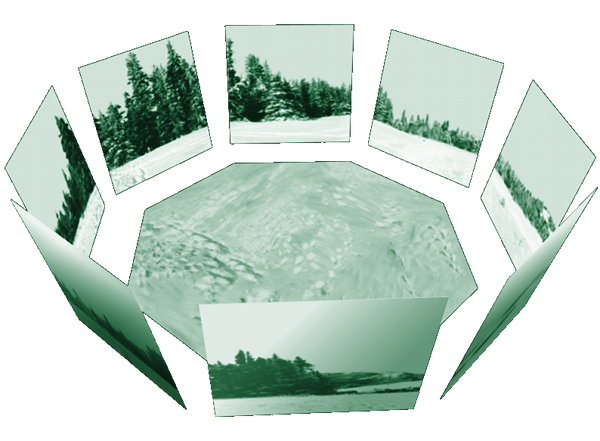
\includegraphics[scale=0.7]{faq_landscape}
%\caption{Figure caption}
\end{figure}

On the negative side, it is more difficult to create this type of
landscape - merging the ground texture with the side textures can prove
tricky. The contents of the \texttt{landscape.ini} file for this
landscape type is also somewhat more complicated than for other
landscape types. Here is the \texttt{landscape.ini} file which describes
the Guereins landscape:

\begin{config}
\texttt{{[}landscape{]}}\\
\texttt{name~=~Guereins}\\
\texttt{type~=~old\_style}\\
\texttt{author~=~Fabien~Chéreau}\\
\texttt{description~=~Guéreins~is~a~small~french~village...}\\
\texttt{nbsidetex~=~8}\\
\texttt{tex0~=~guereins4.png}\\
\texttt{tex1~=~guereins5.png}\\
\texttt{tex2~=~guereins6.png}\\
\texttt{tex3~=~guereins7.png}\\
\texttt{tex4~=~guereins8.png}\\
\texttt{light4~=~guereins8-lgt.png}\\
\texttt{tex5~=~guereins1.png}\\
\texttt{tex6~=~guereins2.png}\\
\texttt{tex7~=~guereins3.png}\\
\texttt{nbside~=~8}\\
\texttt{side0~=~tex0:0:0.005:1:1}\\
\texttt{side1~=~tex1:0:0.005:1:1}\\
\texttt{side2~=~tex2:0:0.005:1:1}\\
\texttt{side3~=~tex3:0:0.005:1:1}\\
\texttt{side4~=~tex4:0:0.005:1:1}\\
\texttt{side5~=~tex5:0:0.005:1:1}\\
\texttt{side6~=~tex6:0:0.005:1:1}\\
\texttt{side7~=~tex7:0:0.005:1:1}\\
\texttt{groundtex~=~guereinsb.png}\\
\texttt{fogtex~=~fog.png}\\
\texttt{nb\_decor\_repeat~=~1}\\
\texttt{decor\_alt\_angle~=~40}\\
\texttt{decor\_angle\_shift~=~-22}\\
\texttt{decor\_angle\_rotatez~=~0}\\
\texttt{ground\_angle\_shift~=~-22}\\
\texttt{ground\_angle\_rotatez~=~45}\\
\texttt{fog\_alt\_angle~=~20}\\
\texttt{fog\_angle\_shift~=~-3}\\
\texttt{draw\_ground\_first~=~1}
\end{config}

Where:

\begin{itemize}
\item
  \textbf{name} is the name that will appear in the landscape tab of the
  configuration window for this landscape
\item
  \textbf{type} should be ``old\_style'' for the multiple image method.
\item
  \textbf{author} lists the author(s) responsible for images and
  composition.
\item
  \textbf{description} gives a short description visible in the
  selection panel. The text will be superseded by optional
  description..utf8 files.
\item
  \textbf{nbsidetex} is the number of side textures for the landscape.
\item
  \textbf{tex0 ... tex} are the side texture file names. These should
  exist in the \texttt{.../textures/landscapes} directory in PNG format.
\item
  \textbf{light0 ... light} are optional textures. If they exist, they
  are used as overlays on top of the respective
  tex\textless{}...\textgreater{} files and represent nocturnal
  illumination, e.g. street lamps, lit windows, red dots on towers, sky
  glow by city light pollution, ... Empty panels don't have to exist. If
  you need your light pollution higher in the sky, you must use a
  spherical or fisheye landscape. (New feature, V0.13.1)
\item
  \textbf{nbside} is the number of side textures
\item
  \textbf{side0 ... side} are the descriptions of how the side textures
  should be arranged in the program. Each description contains five
  fields separated by colon characters (:). The first field is the ID of
  the texture (e.g. tex0), the remaining fields are the texture
  coordinates (x0:y0:x1:y1) used to place the texture in the scene. If
  you want to use all of the image, this will just be \texttt{0:0:1:1}.
\item
  \textbf{groundtex} is the name of the ground texture file. (This could
  also be a diagram e.g. indicating the mountain peaks!)
\item
  \textbf{ground} {[}NO LONGER USED{]} used to be the description of the
  projection of the ground texture in the scene.
\item
  \textbf{fogtex} is the name of the texture file for fog in this
  landscape. Note that for this landscape, accurate overlay of fog and
  landscape is only done if \texttt{calibrated=true} and
  \texttt{tan\_mode=true}.
\item
  \textbf{fog} {[}NO LONGER USED{]} used to be the description of the
  projection of the fog texture in the scene.
\item
  \textbf{nb\_decor\_repeat} is the number of times to repeat the side
  textures in the 360 panorama. (Photo panoramas should have ``1'' here)
\item
  \textbf{decor\_alt\_angle} (degrees) is the vertical angular size of
  the textures (i.e. how high they go into the sky).
\item
  \textbf{decor\_angle\_shift} (degrees) vertical angular offset of the
  scenery textures, at which height are the side textures placed.
\item
  \textbf{decor\_angle\_rotatez} (degrees) angular rotation of the
  scenery around the vertical axis. This is handy for rotating the
  landscape so North is in the correct direction.
\item
  \textbf{ground\_angle\_shift} (degrees) vertical angular offset of the
  ground texture, at which height the ground texture is placed.
\item
  \textbf{ground\_angle\_rotatez} (degrees) angular rotation of the
  ground texture around the vertical axis. When the sides are rotated,
  the ground texture may need to be rotated as well to match up with the
  sides.
\item
  \textbf{fog\_alt\_angle} (degrees) vertical angular size of the fog
  cylinder - how fog looks. Accurate vertical size requires
  \texttt{calibrated=true}.
\item
  \textbf{fog\_angle\_shift} (degrees) vertical angular offset of the
  fog texture - at what height is it drawn. Accurate vertical placement
  requires \texttt{calibrated=true}.
\item
  \textbf{draw\_ground\_first} if 1 the ground is drawn in front of the
  scenery, i.e. the side textures will overlap over the ground texture.
\item
  \textbf{calibrated} (optional, not used in this file). New since
  0.10.6: Only if true, decor\_alt\_angle etc. really work as documented
  above. The (buggy) old code was left to work with the landscapes
  already existing.
\item
  \textbf{tan\_mode} (optional, not used in this file). If true, the
  panorama image must be in in cylindrical, not equirectangular
  projection. Finding \texttt{decor\_alt\_angle} and
  \texttt{decor\_angle\_shift} may be a bit more difficult with this,
  but now (V0.13) works also with calibrated. A fog image created as
  overlay on the pano will be perfectly placed.
\item
  \textbf{decor\_angle\_rotatez} angular rotation of the scenery around
  the vertical axis. This is handy for rotating the landscape so North
  is in the correct direction. If 0, the left edge of \texttt{tex0} is
  due east.
\item
  \textbf{ground\_angle\_shift} vertical angular offset of the ground
  texture, at which height the ground texture is placed. Values above
  -10 are not recommended for non-photographic content due to high
  distortion.
\item
  \textbf{ground\_angle\_rotatez} angular rotation of the ground texture
  around the vertical axis. When the sides are rotated, the ground
  texture may need to be rotated as well to match up with the sides. If
  0, east is up. if North is up in your image, set this to 90.
\item
  \textbf{fog\_alt\_angle} vertical angular size of the fog texture -
  how fog looks.
\item
  \textbf{fog\_angle\_shift} vertical angular offset of the fog texture
  - at what height is it drawn.
\item
  \textbf{draw\_ground\_first} if 1 the ground is drawn before the
  sides, i.e. the side textures may overlap the ground texture if
  \texttt{ground\_angle\_shift\ \&gt;\ decor\_angle\_shift}.
\item
  \textbf{polygonal\_horizon\_list} (optional) is the name of the
  (measured) horizon data file for this landscape. Can be used to query
  horizon transparency (for accurate object rising/setting times)
\item
  \textbf{polygonal\_horizon\_list\_mode} (optional) the two first
  columns in the list are numbers: azimuth and altitude or zenith
  distance, in either degrees or radians or gradians(gon). The value
  must be one of
  azDeg\_altDeg\textbar{}azDeg\_zdDeg\textbar{}azRad\_altRad\textbar{}azRad\_zdRad\textbar{}azGrad\_altGrad\textbar{}azGrad\_zdGrad.
  Default: azDeg\_altDeg
\item
  \textbf{polygonal\_angle\_rotatez} (optional, default=0) Angle
  (degrees) to adjust azimuth. This may be used to apply a (usually)
  small offset rotation, e.g. when you have measured the horizon in a
  grid-based coordinate system like UTM and have to compensate for the
  meridian convergence.
\item
  \textbf{horizon\_line\_color} (optional, default: invisible) used to
  draw a polygonal horizon line.
\item
  \textbf{minimal\_brightness} (optional, default=-1, i.e. use preset
  landscape/minimal\_brightness from global config.ini) Some minimum
  brightness to keep landscape visible.
\item
  \textbf{minimal\_altitude} (optional, default=-2) Some sky elements,
  e.g. stars, are not drawn below this altitude. Under certain
  circumstances you may want to specify something else here. (since
  V0.14)
\end{itemize}

\subsection{landscape.ini {[}location{]}
section}\label{landscape.ini-location-section}

An example location section:

\begin{config}
\texttt{{[}location{]}}\\
\texttt{planet~=~Earth}\\
\texttt{latitude~=~+48d10'9.707"}\\
\texttt{longitude~=~+11d36'32.508"}\\
\texttt{altitude~=~83}\\
\texttt{light\_pollution=3}\\
\texttt{atmospheric\_extinction\_coefficient=0.2}\\
\texttt{atmospheric\_temperature=10}\\
\texttt{atmospheric\_pressure=-1}
\end{config}

Where:

\begin{itemize}
\item
  \textbf{planet} Is the English name of the solar system body for the
  landscape.
\item
  \textbf{latitude} Is the latitude of site of the landscape in degrees,
  minutes and seconds. Positive values represent North of the equator,
  negative values South of the equator.
\item
  \textbf{longitude} Is the longitude of site of the landscape. Positive
  values represent East of the Greenwich Meridian on Earth (or
  equivalent on other bodies), Negative values represent Western
  longitude.
\item
  \textbf{altitude} Is the altitude of the site of the landscape in
  meters.
\item
  \textbf{country} (optional) Name of the country the location is in
\item
  \textbf{state} (optional) Name of the state the location is in
\item
  \textbf{name} (optional) Name of the location
\end{itemize}

Since 0.11, there are a few more optional parameters that can be loaded
if the according switch is active in the landscape selection panel. If
they are missing, the parameters do not change to defaults.

\begin{itemize}
\item
  \textbf{light\_pollution} (optional) Light pollution of the site,
  given on the Bortle Scale (1: none ... 9: metropolitan). If negative
  or absent, no change will be made.
\item
  \textbf{atmospheric\_extinction\_coefficient} (optional, no change if
  absent.) Extinction coefficient (mag/airmass) for this site.
\item
  \textbf{atmospheric\_temperature} (optional, no change if absent.)
  Surface air temperature (Degrees Celsius). Used for refraction. . Set
  to -1000 to explicitly declare ``no change''.
\item
  \textbf{atmospheric\_pressure} (optional, no change if absent.)
  Surface air pressure (mbar; would be 1013 for ``normal'' sea-level
  conditions). Used for refraction. Set to -2 to declare ``no change'',
  or -1 to compute from altitude.
\item
  \textbf{display\_fog} (optional, -1/0/1, default=-1) You may want to
  preconfigure setting \textbf{0} for a landscape on the Moon. Set -1 to
  declare ``no change''.
\end{itemize}

\subsection{Making a Multi panel
Panorama}\label{making-a-multi-panel-panorama}

\begin{figure}[h]
\centering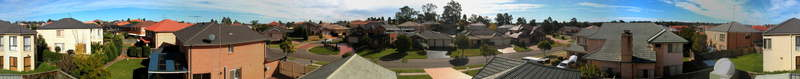
\includegraphics[scale=2.2]{landscape_beaumonthills.jpg}
%\caption{Figure caption}
\end{figure}

This is the only way to get a high resolution panorama and although this
procedure is based on the Microsoft Windows System the basics will apply
to any platform that can run the programs mentioned or similar programs
on the preferred system. If you want a high resolution this is the only
method to use. The first thing needed for a personalised landscape to
superimpose on the horizon display is a 360$\degree$ panorama with a transparent
background. To make this you will need the following:

\begin{itemize}
\item
  A digital camera on a tripod or stable platform
\item
  A program to convert the pictures into a 360$\degree$ panorama
\item
  A program to remove the background and convert the panorama into about
  8 square pictures in PNG format for insertion into Stellarium as the
  sides and if possible a similar square picture of the base you are
  standing on to form the ground. This last requirement is only really
  possible if this area is relatively featureless as the problem of
  knitting a complex base is well nigh impossible.
\item
  Patience. (Maybe a soundproof room so that the swearing wont be heard
  when you press the wrong key and lose an hours work)
\end{itemize}

\subsubsection{The Camera}\label{the-camera}

Digital cameras are easy and cheaply available these days so whatever
you have should do. One mega-pixel resolution is quite sufficient.

The camera needs to be mounted on a tripod so that reasonably orientated
pictures can be taken. Select a time of day that is quite bright with a
neutral cloudy sky so there will be no shadows and a sky of the same
overall texture. This will make it easier to remove later. The pictures
were all saved in the JPG format which was used as the common format for
all processes up to the removal of the background.

With a camera that takes 4:3 ratio pictures I found 14 evenly spaced
pictures gave the best 360$\degree$ panorama in the program I used to produce
it.

\subsubsection{Processing into a
Panorama}\label{processing-into-a-panorama}

This is the most complicated part of the process of generating the
panorama. I used two separate programs to do this. Firstly I used The
Gimp to re size the panels to 1024x768 and so make them easier to handle
in the panorama program.

When I had my 14 processed pictures I inserted them into the panorama
program. I first used a program called the Panorama Factory. Version 1.6
is a freebee that works well and can be downloaded from the internet - a
Google search will find it. I later used version 3.4 that is better and
cost about \$40 off the Internet. This program has many options and can
be configured to suit most cameras and can make a seamless 360$\degree$ panorama
in barrel form that will take a highly trained eye to find where the
joins occur.

The resulting panorama was then loaded into The Gimp and trimmed to a
suitable size. Mine ended up 14024 x 1601 pixels. I trimmed the vertical
size to 1024 by cutting back then stretched the 14024 to 14336 pixels,
with almost no distortion, that would allow cutting into 14 1024 x1024
pictures at a later date. If the height of the panorama had been greater
I could have made fewer pictures and so shown more of the foreground.
See figure {[}fig:panorama360{]}.

If you have prominent foreground items like posts wires etc. that occur
in adjacent pictures the panorama program will have difficulty in
discerning them because of the 3D effect and may give double images. I
overcame this by painting out the offending item by cut and paste
between the two pictures. Quite easy with a little practice using the
zoom in facility and I found the MSpaint program the easiest to do this
in.

\begin{figure}[h]
\centering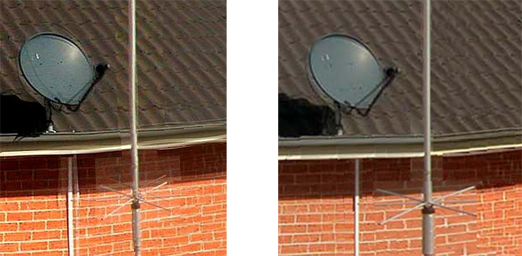
\includegraphics[scale=2.0]{BEAU-3c}
%\caption{Figure caption}
\end{figure}

\subsubsection{Removing the background to make it
transparent}\label{removing-the-background-to-make-it-transparent}

This is the most complex part of the process and requires a program that
can produce transparency to parts of your picture, commonly called an
alpha channel. Two programs I know of will do this. The very expensive
and sophisticated Adobe Photoshop and a freebee called The Gimp. I used
photoshop to cut the full panorama into 1024 x 1024 textures because it
was the easiest to do accurate cutting but it can be done in TheGimp as
well.

I first used Photoshop to produce the alpha channel because it was the
only way I knew but I now use the GIMP as it is much easier to process
the individual textures than removing the background from the full
panorama.

\begin{enumerate}
\item
  Load the 1st section into TheGimp
\item
  Next create a new empty picture 1024 x 1024 then use the advanced tab
  to make the background color transparency. Copy the original texture
  onto this new picture base so that it exactly fits the frame then
  select layer from the menu and press anchor. This will create a new
  picture with with an alpha channel. By using the select by color and
  lasso etc cut out the parts you don't want this will expose the
  checkerboard background. When you are happy with the removal save the
  texture in *.png format to preserve the alpha layer.
\item
  Do the same with the remaining pictures to make all the components of
  the landscape.
\item
  Make a new directory for the landscape. This should be a sub-directory
  of either the /landscapes or /landscapes directory. The name of the
  directory should be unique to your landscape, and is the landscape ID.
  The convention is to use a single descriptive word in lowercase text,
  for example gueriens. Place your pictures your new directory.
\item
  In your new landscape directory, create a new file called
  landscape.ini file (I used wordpad). Add a line for the
  {[}landscape{]} section. It's probably easiest to copy the
  landscape.ini file for the Gueriens landscape and edit it. Edit the
  name Guereins in every instance to the name you have given your
  landscape. Don't forget to make the number of tex entries agree with
  the number of your pictures. If you haven't made a groundtex picture
  use one of the existing ones from the file or make a square blank
  picture of your own idea. Because I took my pictures from the roof of
  the house I used an edited picture of the roof of my house from Google
  Earth. It was pretty cruddy low resolution but served the purpose.
\item
  Next you need to orientate your picture North with true North. This is
  done roughly by making the arrangement of side1 to siden suit your
  site as close as possible. Now you need to edit the value of
  decor\_angle\_rotatez to move your landscape in azimuth. Edit
  decor\_alt\_angle to move you landscape in altitude to align your
  visible horizon angle. Edit ground\_angle\_rotatez to align your
  ground with the rest of the landscape. Leave the other entries they
  are suitable as is.
\end{enumerate}

After re-starting Stellarium, your landscape will appear in the
landscape folder of the main menu , and can be selected as required.

\subsection{Making a Spherical
Panorama}\label{making-a-spherical-panorama}

A simpler method of making a panorama is to use the spherical method.
These can be made to create the full panorama using the program
Autostitch. The big advantage of the spherical panorama is that it does
not need a ground panel. However the drawback with the Spherical
panorama is that few computer video cards will reproduce a panorama
larger than 4096 x 2048 pixels and many will not do better than 2048 x
1024 pixels

\begin{figure}[h]
\centering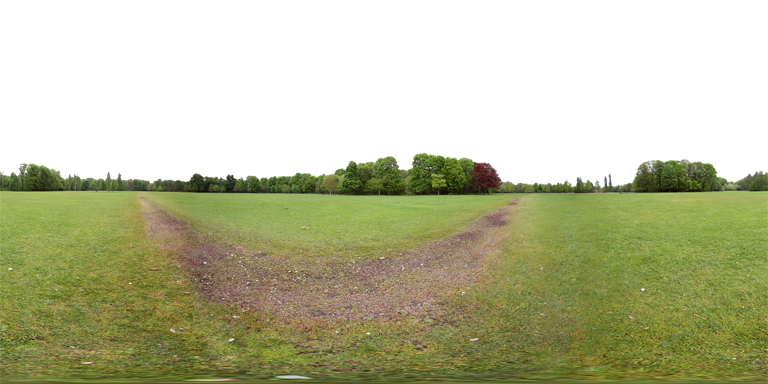
\includegraphics{egarden}
%\caption{Figure caption}
\end{figure}

The Autostitch program is quite easy to use. Make sure your panorama
shots take the ground almost up to your feet and follow the instructions
in the readme file. \href{http://www.example.com}{link title} When the
panorama is finished it will be in *,jpg format. This will need to be
converted to a *.png with transparent background (alpha layer) and have
the sky removed. This can be done in TheGimp as in the multi-panel type.
When the sky is removed make sure you save the landscape in *.png
format.

My computer will only do 2048 by 1024, If I try to load a larger type I
just get a white screen. With this problem I used the following
procedure to make the spherical into a four panel multi-panel landscape
with a very effective ground that matched well

\subsubsection{Converting a Spherical Panorama into a Multi
Panel}\label{converting-a-spherical-panorama-into-a-multi-panel}

Most computers with standard video cards will not display spherical
panoramas larger than 4096 x 2048 and some will not even go beyond 2048
x 1024. This makes rather poor resolution panaoramas. OK for planets but
not very pretty for your local environment. If the panorama can have a
horizontal section cut out that can keep the detail within a 1024
vertical boundary it is ideal for processing into 1024 x 1024 sections.
When you have the sections proceed as with the previous description

\begin{figure}[h]
\centering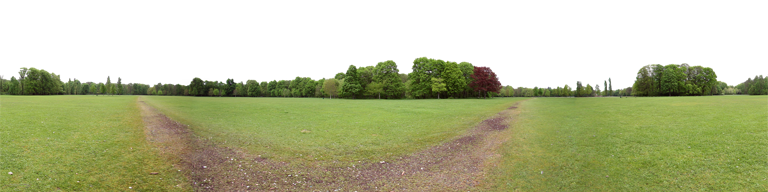
\includegraphics{egarden-narrow}
%\caption{Figure caption}
\end{figure}

I made the egarden into a 4096 x 1024 quite easily because there was a
lot of blank space above the horizon. This would allow 4 panels 1024 x
1024 pixels.in fact if I had a 8192 x 4096 panorama I could have made it
into 8 1024 x 1024 panels. This would have given me quite a high
resolution horizon

\begin{figure}[h]
\centering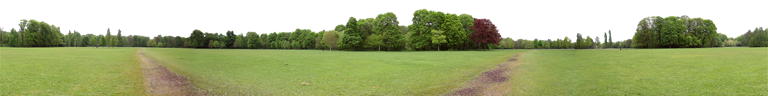
\includegraphics{egarden-narrow-2}
%\caption{Figure caption}
\end{figure}


\begin{enumerate}
\item
  Load the sections into TheGimp and process them into 1024 x 1024
  textures with alpha layers as before.
\item
  Next use a 2048 x 1024 version of the panorama in Stellarium. Drag the
  screen around so it produces a centralised picture on the Stellarium
  screen of the ground at the highest resolution possible and take a
  screen shot. This screen shot can be then processed into a quite
  effective ground texture in TheGimp that can be adjusted to match the
  rest of the panorama.
  \begin{figure}[h]
  \centering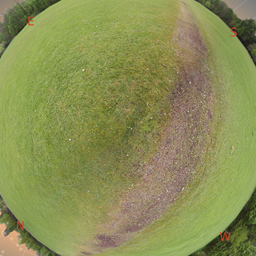
\includegraphics[scale=2.0]{egardembase}
  %\caption{Figure caption}
  \end{figure}
\item
  Make a new directory etc. for the landscape.
\item
  You can make it fit using the variablein the landscape.ini file
  decor\_alt\_angle=xx decor\_angle\_shift=xx and
  decor\_angle\_rotatez=xx.Then the ground can be matched with
  ground\_angle\_shift=xx and ground\_angle\_rotatez=xx.
\item
  Make sure the draw\_ground\_first=1 to ensure that the main panorama
  overplays the ground
\end{enumerate}

After re-starting Stellarium, your landscape will appear in the
landscape tab of the main menu, and can be selected as required.

When the panorama is finished it will be in *.jpg format. It will need
to be converted to a *.png with transparent background (alpha layer) and
have the sky removed. This is done in TheGimp as in the multipanel type.
When the sky is removed make sure you save the landscape in *.png
format.

The drawback with the spherical panorama is that few computer video
cards will reproduce a panorama larger than 4096 x 2048 pixels in
Stellarium and many will not do better than 2048 x 1024 pixels.

My computer will only do 2048 by 1024, If I try to load a larger type I
just get a white screen. With this problem I used the following
procedure to make the spherical into a four panel multi panel landscape
with a very effective ground that matched well.

\subsection{Making a Fish eye
Panorama}\label{making-a-fish-eye-panorama}

This sort of panorama needs a very expensive fisheye lens on your
camera. It is really only practical for a planetarium display to give a
simple more or less silouette landscape where the ground is completely
obscured. It can only be used with quite small pictures of no more than
1024 x 1024 pixels. Once you have your fisheye texture it must still be
processed in TheGimp to remove the sky and convert into an alpha layer
texture

\begin{figure}[h]
\centering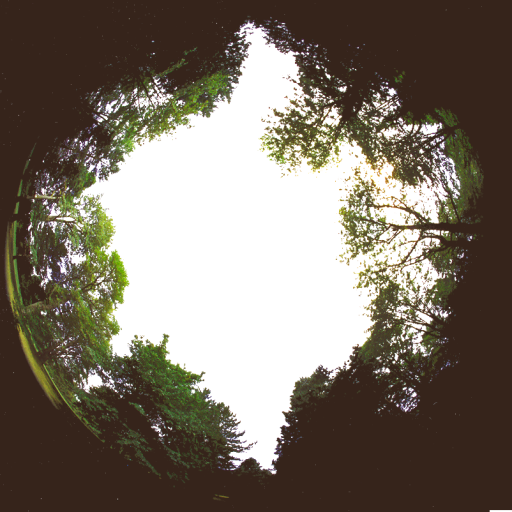
\includegraphics[scale=3.0]{trees_512}
%\caption{Figure caption}
\end{figure}

The sample supplied with Stellarium is called trees. The horizon needs
to be identified and the picture sized so that the panorama above the
horizon is sited to be about 80\% of the total extent and the the
balance of the border filled with a dark colour right up to the horizon.
This will make the horizon in your landscape at 0 degrees.

It is possible to make a synthetic fisheye texture using the same method
as making a ground from a spherical panorama but it is hardly worth the
trouble as even a simple 2048 x 1024 pixel sperical will give a far
better result.

\section{Deep-Sky Objects}\label{deep-sky-objects}

Extended objects are those which are external to the solar system, and
are not point-sources like stars. Extended objects include galaxies,
planetary nebulae and star clusters. These objects may or may not have
images associated with them. Stellarium also comes with a catalogue with
over 14,000 extended objects containing the combined data from many
catalogues, with 190 images.

Since to version 0.10.0 Stellarium uses new method of displaying
textures using the ``json'' cataloguing system. At the same time the
Simbad online catalogue was added to the search feature making it
largely redundant and used now only as a first search point or if there
is no internet connection.

If the object has a name (not just a catalogue number), you should add
one or more records to the \texttt{.../nebulae/default/names.dat} file
(where \texttt{...} is either the installation directory or the user
directory). See section
\emph{\protect\hyperlink{Modifyingux5fnames.dat}{Modifying names.dat}}
for details of the file format.

If you wish to associate a texture (image) with the object, you must now
add a record to the \texttt{.../nebulae/default/textures.json} file. See
section \emph{\protect\hyperlink{Modifyingux5ftextures.json}{Modifying
textures.json}} for details of the file format.

Nebula images should have dimensions which are integer powers of two,
i.e. 1, 2, 4, 8, 16, 32, 64, 128, 256, 512, 1024 ... pixels along each
side. If this requirement is not met, your textures may not be visible,
or graphics performance may be seriously impacted. PNG or JPG formats
are both supported.

\subsection{GUI for manage by Deep-Sky
Objects}\label{gui-for-manage-by-deep-sky-objects}

\begin{figure}[h]
\centering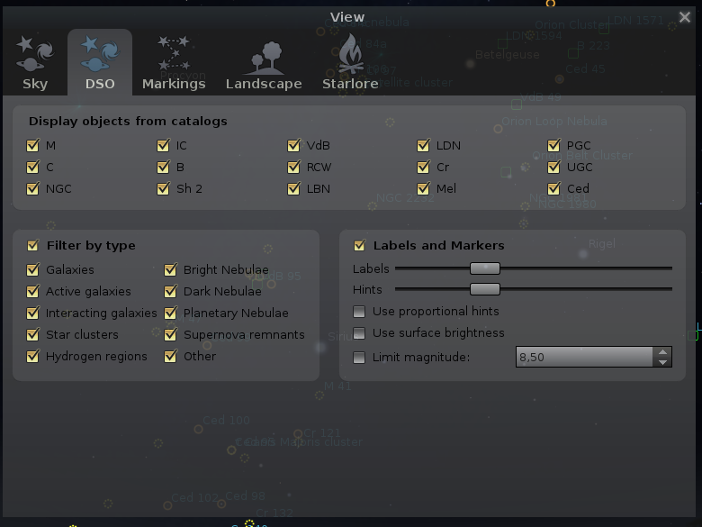
\includegraphics{DSO_GUI}
%\caption{Figure caption}
\end{figure}

\subsection{Stellarium DSO Catalog}\label{stellarium-dso-catalog}

Stellarium DSO Catalog is contains over 1400 objects and he available
for end users as collection of files:

\begin{itemize}
\item
  \texttt{catalog.txt} - Stellarium DSO Catalog in ASCII format for
  editing data;
\item
  \texttt{catalog.dat} - Stellarium DSO Catalog in binary format for
  usage within Stellarium;
\item
  \texttt{names.dat} - list of proper names of the objects from
  \texttt{catalog.dat} file.
\end{itemize}

ASCII file can be converted into binary format through enabling option
\texttt{devel/convert\_dso\_catalog\ =\ true} in the \texttt{config.ini}
file. The file \texttt{catalog.txt} should be put to the directory
\texttt{.../nebulae/default/}.

Stellarium DSO Catalog contains data and supported the designations for
follow catalogues:

\begin{itemize}
\item
  New General Catalogue (NGC)
\item
  Index Catalogue (IC)
\item
  Messier Catalog (M)
\item
  Caldwell Catalogue (C)
\item
  Barnard Catalogue (B)
\item
  Sharpless Catalogue (Sh2)
\item
  Van den Bergh Catalogue of reflection nebulae (VdB)
\item
  A catalogue of H$\alpha$-emission regions in the southern Milky Way (RCW)
\item
  Lynds' Catalogue of Dark Nebulae (LDN)
\item
  Lynds' Catalogue of Bright Nebulae (LBN)
\item
  Collinder Catalogue (Cr)
\item
  Melotte Catalogue of Deep Sky Objects (Mel)
\item
  HYPERLEDA. I. Catalog of galaxies (PGC)\footnote{Partial support}
\item
  The Uppsala General Catalogue of Galaxies (UGC)\footnote{Partial
    support}
\item
  Cederblad Catalog of bright diffuse Galactic nebulae (Ced)
\end{itemize}

\subsection{Modifying catalog.dat}\label{modifying-catalog.dat}

This section is described inner structure of files \texttt{catalog.dat}
(has binary format) and \texttt{catalog.txt} (has ASCII format).
Stellarium can convert ASCII file into the binary format file for usage
within planetarium.

Each line contains one record, each record consisting of the following
fields with \emph{tab} char as delimiter:

\begin{longtabu} to \textwidth {l|l|X}
\toprule
\emph{Column} & \emph{Type} & \emph{Description}\tabularnewline
\midrule
1 & integer & Deep-Sky Object Identificator\tabularnewline
2 & float & RA (decimal degrees)\tabularnewline
3 & float & Dec (decimal degrees)\tabularnewline
4 & float & B magnitude\tabularnewline
5 & float & V magnitude\tabularnewline
6 & string & Object type (Possible values see in table
\emph{\protect\hyperlink{Typesux5fofux5fObjects}{Types of
Objects}}).\tabularnewline
7 & string & Morphological type of object\tabularnewline
8 & float & Major axis size or radius (arcmin)\tabularnewline
9 & float & Minor axis size (arcmin)\tabularnewline
10 & integer & Orientation angle (degrees)\tabularnewline
11 & float & Redshift\tabularnewline
12 & float & Error of redshift\tabularnewline
13 & float & Parallax (mas)\tabularnewline
14 & float & Error of parallax (mas)\tabularnewline
15 & float & Non-redshift distance (Mpc for galaxies, kpc for other
objects)\tabularnewline
16 & float & Error of non-redsift distance (Mpc for galaxies, kpc for
other objects)\tabularnewline
17 & integer & NGC number (New General Catalogue)\tabularnewline
18 & integer & IC number (Index Catalogue)\tabularnewline
19 & integer & M number (Messier Catalog)\tabularnewline
20 & integer & C number (Caldwell Catalogue)\tabularnewline
21 & integer & B number (Barnard Catalogue)\tabularnewline
22 & integer & Sh2 number (Sharpless Catalogue)\tabularnewline
23 & integer & VdB number (Van den Bergh Catalogue of reflection
nebulae)\tabularnewline
24 & integer & RCW number (A catalogue of H$\alpha$-emission regions in the
southern Milky Way)\tabularnewline
25 & integer & LDN number (Lynds' Catalogue of Dark
Nebulae)\tabularnewline
26 & integer & LBN number (Lynds' Catalogue of Bright
Nebulae)\tabularnewline
27 & integer & Cr number (Collinder Catalogue)\tabularnewline
28 & integer & Mel number (Melotte Catalogue of Deep Sky
Objects)\tabularnewline
29 & integer & PGC number (HYPERLEDA. I. Catalog of galaxies);
partial\tabularnewline
30 & integer & UGC number (The Uppsala General Catalogue of Galaxies);
partial\tabularnewline
31 & string & Ced number (Cederblad Catalog of bright diffuse Galactic
nebulae)\tabularnewline
\bottomrule
\end{longtabu}

\subsubsection{Types of Objects}\label{types-of-objects}

Possible values for type of objects in the file \texttt{catalog.dat}.

\begin{longtabu} to \textwidth {l|X}
\toprule
\emph{Type} & \emph{Description}\tabularnewline
\midrule
G & Galaxy\tabularnewline
GX & Galaxy\tabularnewline
AGX & Active Galaxy\tabularnewline
RG & Radio Galaxy\tabularnewline
IG & Interacting Galaxy\tabularnewline
GC & Globular Cluster\tabularnewline
OC & Open Cluster\tabularnewline
NB & Nebula\tabularnewline
PN & Planetary Nebula\tabularnewline
DN & Dark Nebula\tabularnewline
RN & Reflection Nebula\tabularnewline
C+N & Cluster associated with nebulosity\tabularnewline
HII & HII Region\tabularnewline
SNR & Supernova Remnant\tabularnewline
BN & Bipolar Nebula\tabularnewline
EN & Emission Nebula\tabularnewline
SA & Stellar Association\tabularnewline
SC & Star Cloud\tabularnewline
CL & Cluster\tabularnewline
IR & Infra-Red Object\tabularnewline
QSO & Quasar\tabularnewline
Q? & Possible Quasar\tabularnewline
ISM & Interstellar Matter\tabularnewline
EMO & Emission Object\tabularnewline
LIN & LINEAR-type Active Galaxies\tabularnewline
BLL & BL Lac Object\tabularnewline
BLA & Blazar\tabularnewline
MOC & Molecular Cloud\tabularnewline
YSO & Young Stellar Object\tabularnewline
PN? & Possible Planetary Nebula\tabularnewline
PPN & Protoplanetary Nebula\tabularnewline
$\ast$ & Star\tabularnewline
$\ast\ast$ & Double Star\tabularnewline
MUL & Multiple Star\tabularnewline
\emph{empty} & Unknown type, catalog errors, \emph{Unidentified Southern
Objects} etc.\tabularnewline
\bottomrule
\end{longtabu}

\subsection{Modifying names.dat}\label{modifying-names.dat}

Each line in the \texttt{names.dat} file contains one record. A record
relates an extended object catalogue number (from \texttt{catalog.dat})
with a name. A single catalogue number may have more than one record in
this file.

The record structure is as follows:

\begin{longtabu} to \textwidth {l|l|l|X}
\toprule
\emph{Offset} & \emph{Length} & \emph{Type} & \emph{Description}\tabularnewline
\midrule
0 & 5 & \%5s & Designator for catalogue (prefix)\tabularnewline
5 & 15 & \%d & Identificator for object in the catalog\tabularnewline
20 & 60 & \%s & Proper name of the object (translatable)\tabularnewline
\bottomrule
\end{longtabu}

If an object has more than one record in the \texttt{names.dat} file,
the last record in the file will be used for the nebula label.

\subsection{Modifying textures.json}\label{modifying-textures.json}

This file is used to describe each nebula image. The file structure
follows the JSON format, a detailed description of which may be found at
. The textures.json file which ships with Stellarium has the following
structure:

\begin{itemize}
\item
  serverCredits (optional) - a structure containing the following
  key/value pairs:

  \begin{itemize}
  \item
    short - a short identifier of a server where the json file is found,
    e.g. ``ESO''
  \item
    full - a longer description of a server, e.g. ``ESO Online Digitised
    Sky Survey Server''
  \item
    infoURL - a URL pointing at a page with information about the server
  \end{itemize}
\item
  imageCredits - a structure containing the same parts as a
  serverCredits structure but referring to the image data itself
\item
  shortName - an identifier for the set of images, to be used inside
  Stellarium
\item
  minResolution - minimum resolution, applies to all images in the set,
  unless otherwise specified at the image level
\item
  maxBrightness - the maximum brightness of an image, applies to all
  images in the set, unless otherwise specified at the image level
\item
  subTiles - a list of structures describing indiviual image tiles, or
  referring to another json file. Each subTile may contain:

  \begin{itemize}
  \item
    minResolution
  \item
    maxBrightness
  \item
    worldCoords
  \item
    subTiles
  \item
    imageCredits
  \item
    imageUrl
  \item
    textureCoords
  \end{itemize}
\item
  shortName (name for the whole set of images, e.g. ``Nebulae'')
\item
  miniResolution (applies to all images in set)
\item
  alphaBlend (applies to all images in set)
\item
  subTiles list of images. Each image record has the following
  properties:

  \begin{itemize}
  \item
    imageCredits (itself a list of key/pairs)
  \item
    imageUrl (e.g. file name)
  \item
    worldCoords (a list of four pairs of coordinates representing the
    corners of the image)
  \item
    textureCoords (a list of four pairs of corner descriptions. i.e.
    which is top left of image etc)
  \item
    minResolution (over-rides file-level setting)
  \item
    maxBrightness
  \end{itemize}
\end{itemize}

Items enclosed in Quotation marks are strings for use in the program.
Syntax is extremely important. Look at the file with a text editor to
see the format. Items in \textless{}\textgreater{} are user provided
strings and values to suit the texture and source.

\texttt{Line~1~“imageCredits”:~\{“short”~:~“}\texttt{”~:~“infoUrl”:~}\href{http://}{\texttt{http://}}\texttt{\},~}\\
\texttt{Line~2~“imageUrl”~:~“}\texttt{”,~}\\
\texttt{Line~3~“worldCoords”~:~\textless{}~decimal~numerical~values~of~the~J2000~coordinates~of~the~corners~of~the~texture~\textgreater{}~These~values~displayed~to~4~decimal~places~in~the~format~of~the~texture~coordinates~}\\
\texttt{Line~4~“textureCoords”~:~{[}{[}{[}~0,0{]},{[}1,0{]},{[}1,1{]},{[}0,1{]}{]}{]},~Where~0,0~is~South~Left~,~1,0~the~South~Right~,~1,1~North~Right~,~0,1~North~Left~corners~of~texture~Format~=~RA~in~degrees,~Dec~in~degrees~}\\
\texttt{Line~5~“MinResolution”~:~}\texttt{,~}\\
\texttt{Line~6~“maxBrightness”~:~\textless{}~a~numerical~vale~representing~the~absolute~brightness~for~the~display\textgreater{}~}

Calculating of the coords of the corners of the images (plate solving)is
a time consuming project and needs to be fine tuned from the screen
display. As most images will be two dimensional, display on a spherical
display will limit the size to about 1 degree before distortion becomes
evident. Larger displays can be sectioned into a mosaic of smaller
textures for a more accurate display

\subsection{Adding Extra Nebulae
Images}\label{adding-extra-nebulae-images}

\subsubsection{\texorpdfstring{Preparing a photo for inclusion to the
\texttt{textures.json}
file}{Preparing a photo for inclusion to the textures.json file}}\label{preparing-a-photo-for-inclusion-to-the-textures.json-file}

\begin{figure}[h]
\centering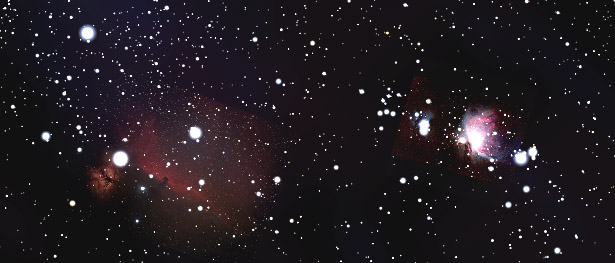
\includegraphics{nebula-display}
\caption{Screen shot of nebula images displayed in Stellarium}
\end{figure}

The first step is to take a photo of the object you wish to display in
Stellarium as a screen backdrop. Then when you have the picture you will
need align it so that north is directly up and not inverted side to side
or up and down as can happen with photos taken with a diagonal mirror in
the path. Next you will need to crop the picture, setting the main
feature at the centre and making the cropped size a factor of 2n eg. 64,
128, 256, 512 or 1024 pixels square. When cropping make sure you leave
at least five prominent background stars

The next step is to process your photo to make the background
black,black. This will ensure that your background will meld with the
Stellarium background and not be noticed. Suitable programs to do all
this are The Gimp (free in keeping with the Stellarium spirit) or
Photoshop if you can afford it.

When you have your prepared image you will need to plate solve it using
at least 6 known GSC stars that can be identified. That is why the
cropping with plenty of stars was necessary. When the plate is solved
you will need to find the J2000 coordinates of the corners and convert
them to decimal values to form the world coordinates in the
\texttt{textures.json} file.

\begin{figure}[h]
\centering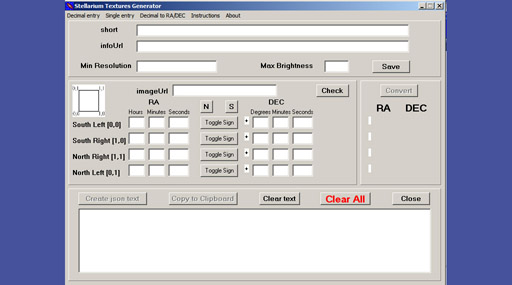
\includegraphics{EQ-Decimal.jpg}
\caption{A program to convert Equatorial coordinates into decimal
form and write a \texttt{textures.json} insert}
\end{figure}

The program in the picture can accept the corner coordinates of a
texture in your plate solving program into decimal values and write an
insert for the \texttt{textures.json} file. It is available as a freebee
from
\url{http://www.madpc.co.uk/~peterv/astroplover/equipnbits/Stellariumtextures.zip}

\begin{figure}[h]
\centering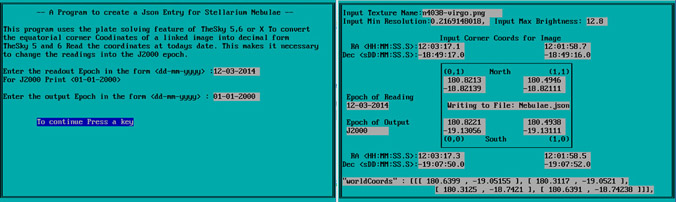
\includegraphics{pix-4.jpg}
\end{figure}

Here is a second program written in Qb64(gl)that will perform the same
task but allow manipulation of the epochs.
\url{http://barry.sarcasmogerdes.com/stellarium/uploads/writejsoninsert.zip}

\subsubsection{Plate Solving}\label{plate-solving}

Suitable programs that can accept your picture and calculate its corner
coordinates are hard to find. I have only found one that suits our
purpose and it is another expensive planetarium program, TheSkyX Pro.
However the older versions TheSky5 and 6 Pro will also do the job if
suitably configured although I could not solve the test program with the
TheSky6 that uses the same procedure as TheSky5 .

These programs have a link feature that can match your photo to the
selected area of the screen and superimpose it on the display with a box
around your photo provided it can match at least 6 stars from the GSC
that is included with the program. When this is fitted you can read the
corner coordinates of your texture in the Status bar by selecting them
with a mouse. TheSkyX can read these coordinates in J2000 values and
uses textures in the fits format but the earlier programs only read the
coordinates of the current program date. To read the J2000 coordinates
it is necessary to re start the program with the date set to 1-1-2000

To add the picture to TheSky5 you need first make a mono 8 bit version
of the photo and place it on the clipboard. Run TheSky and centre on the
object centre. Look in the Tools menu for the image link and select
setup. Tick show image frame to put a frame around the image.

Paste the clipboard image on the display and use the zoom and position
controls to get it as close to the size and position as possible by
visually matching stars. Go to the menu again and click on link wizard.
If you have been successful the window will show the number of stars
matched and the option to accept or continue. Accept and you will now
see all the matched stars have overlaid the picture. You can now read
off the corner coordinates from the status bar starting at the bottom
(south) left and continuing counter clockwise to the top (north) left.

\subsubsection{\texorpdfstring{Processing into a \texttt{textures.json}
insert}{Processing into a textures.json insert}}\label{processing-into-a-textures.json-insert}

Place your image in the \texttt{*.png} format in the
\texttt{.../nebulae/default/} folder. Ensure that the name matches the
\texttt{textures.json} entry.

Once you have the corner coordinates of your photo you can add them to
the decimal converter program and it will write an insert
\texttt{nebula.json} as a text file that you can paste directly into the
\texttt{textures.json} file that is in the \texttt{.../nebulae/default/}
folder.

Save the \texttt{textures.json} file with the new insert and run
Stellarium. Select the object in the Object selection window and slew to
it. Your image should be there and with a bit of luck it will nicely
overlay the stars in the Stellarium program. However this only rarely
happens so a little bit of tweaking of the json worldcoords will be
needed to get a perfect match. Select the telescope (equatorial mode).
This will show the area with north up. Select each corner in sequence
and make small changes to the coordinates. Re start Stellarium each time
and check if you have moved the right direction. Continue with each
corner until all the stars match. With a little bit of practice this
will be done in about 10 minutes.


